\documentclass[a4,center,fleqn]{NAR}

% Enter dates of publication
\copyrightyear{2017}
\pubdate{** ***** ****}
\pubyear{2017}
\jvolume{**}
\jissue{**}

%\articlesubtype{This is the article type (optional)}

\begin{document}

\title{OneD: increasing reproducibility of Hi-C Samples with abnormal
karyotypes}

\author{%
Enrique Vidal\,$^{1,2,*}$,
Fran\c{c}ois le Dily\,$^{1,2}$,
Javier Quilez\,$^{1,2}$,
Ralph Stadhouders\,$^{1,2}$,
Yasmina Cuartero\,$^{1,2,3}$,
Thomas Graf\,$^{1,2}$,
Marc A.  Marti-Renom\,$^{1,2,3,4}$,
Miguel Beato\,$^{1,2}$,
and Guillaume J. Filion\,$^{1,2}$%
\footnote{To whom correspondence should be addressed.
Tel: +34 93 316 01 15; Fax: +34 93 316 00 99; Email: enrique.vidal@crg.eu}}

\address{%
$^{1}$Gene Regulation, Stem Cells and Cancer Program, Centre for
Genomic Regulation (CRG), The Barcelona Institute of Science and
Technology (BIST), Dr. Aiguader 88, 08003, Barcelona, Spain
and
$^{2}$Universitat Pompeu Fabra (UPF), Barcelona, Spain
and
$^{3}$CNAG-CRG, Centre for Genomic Regulation (CRG), Barcelona
Institute of Science and Technology (BIST), Baldiri i Reixac 4, 08028
Barcelona, Spain
and
$^{4}$ICREA, Pg. Llu\'is Companys 23, 08010 Barcelona, Spain}

% Affiliation must include:
% Department name, institution name, full road and district address,
% state, Zip or postal code, country

\history{%
Received January 1, ****;
Revised February 1, ****;
Accepted March 1, ****}

\maketitle

\begin{abstract}
The three-dimensional conformation of genomes is an
essential component of their biological activity. The advent of the Hi-C
technology enabled an unprecedented progress in our understanding of
genome structures. However, Hi-C is subject to systematic biases that can
compromise downstream analyses. Several strategies have been proposed to
remove those biases, but the issue of abnormal karyotypes received little
attention. Many experiments are performed in cancer cell lines, which
typically harbor large-scale copy number variations that create visible
defects on the raw Hi-C maps. The consequences of these widespread
artifacts on the normalized maps are mostly unexplored.
We observed that current normalization methods are not robust to the
presence of large-scale copy number variations, potentially obscuring
biological differences and enhancing batch effects. To address this issue,
we developed an alternative approach designed to take into account
chromosomal abnormalities. The method, called \textit{OneD}, increases
reproducibility among replicates of Hi-C samples with abnormal karyotype,
outperforming previous methods significantly. On normal karyotypes,
\textit{OneD} fared equally well as state-of-the-art methods, making it a
safe choice for Hi-C normalization.  \textit{OneD} is fast and scales well
in terms of computing resources for resolutions up to 5~kbp.
%\textit{OneD} is implemented as an R package
%available at http://www.github.com/qenvio/dryhic.
\end{abstract}


\section{Introduction}

One of the crown achievements of modern biology was to realize that
genomes have an underlying three-dimensional structure contributing to
their activity \citep{rowley2016three, dekker20163d, pezic2017more}. In
mammals, this organization plays a key role in guiding enhancer-promoter
contacts \citep{de2013topology}, in V(D)J recombination
\citep{choi2014ctcf} and in X chromosome inactivation \citep{galupa2015x}.
A significant breakthrough towards this insight was the development of
the high throughput chromosomal conformation capture technology (Hi-C),
assaying chromosomal contacts at a genome-wide scale
\citep{lieberman2009comprehensive}. Nowadays, exploring the spatial
organization of chromatin has become a priority in many fields and Hi-C
has become part of the standard molecular biology toolbox
\citep{dekker2013exploring}.

Contrary to the precursor technologies 3C, 4C and 5C
\citep{dekker2002capturing, simonis2006nuclear,
dostie2006chromosome,de2012decade}, Hi-C interrogates all possible
pairwise interactions between restriction fragments. However, this does
not guarantee that the method has no bias.  On the contrary, local genome
features such as the G+C content, the availability of restriction enzyme
sites and the mappability of the sequencing reads have been shown to
impact the results \citep{yaffe2011probabilistic}, in addition to general
experimental biases such as batch effects. It is thus important to
normalize Hi-C data in order to remove biases and artifacts, so that they
are not confused with biological signal.

Several methods have been proposed to remove biases in Hi-C experiments
\citep{schmitt2016genome}. The first strategy is to model biases
explicitly from a defined set of local genomic features, such as the G+C
content. This approach is used in the method of
\cite{yaffe2011probabilistic} and in Hicnorm by \cite{hu2012hicnorm}. The
second strategy is to implicitly correct unknown biases by enforcing some
regularity condition on the data. This approach is used in the
Iterative Correction and Eigenvector decomposition method (\textit{ICE})
of \cite{imakaev2012iterative}, whereby the total amount of contacts of
every bin is imposed to be the same. \textit{ICE} is currently the most
popular method, due in part to its speed.

Neither of these strategies were designed for cell types with karyotypic
aberrations, most common in cancer. Yet, Hi-C is very sensitive to
aneuploidy, copy number variations and translocations.  Actually, these
aberrations have so much influence on the outcome that they can be used as
signature to re-assemble the target genome \citep{korbel2013genome}. An
additional complication is that karyotypic aberrations are not
experimental biases, so it is unclear whether they should be corrected at
all or be considered part of the biological signal.

% **************************************************************
% Keep this command to avoid text of first page running into the
% first page footnotes
\enlargethispage{-65.1pt}
% **************************************************************

So far, the only attempt to address the issue was the chromosome-adjusted
Iterative Correction Bias method (\textit{caICB}) of
\cite{wu2016computational}. However, \textit{caICB} applies a uniform
chromosome-wide copy number correction, effectively excluding the numerous
cases of partial aneuploidy and regional copy number variations.

Here we propose \textit{OneD}, a method to correct local chromosomal
abnormalities in Hi-C experiments. \textit{OneD} explicitly models the
contribution of known biases via a generalized additive model. The
normalized data is more reproducible between replicates and across
different protocols. Importantly, \textit{OneD} is also efficient when
cells have a normal karyotype, where it performs as well as the best
normalization methods. Finally, the implementation is as fast as
\textit{ICE} and it scales up to 5~kbp resolution with reasonable
computing resources.


\section{MATERIALS AND METHODS}

\subsection{Model}

The most common representation of Hi-C data is a contact matrix, obtained
by slicing the genome in $n$ consecutive bins of fixed size (the
resolution) and computing the number of contacts between each pair of
bins. The values are stored in the cells of the contact matrix ($x_{ij}$),
quantifying the interaction between the two loci at positions $i$ and
$j$.

Our approach is to model the tally of contacts for each bin, thus reducing
the matrix to a one dimension score (hence the name \textit{OneD}). We
assume that the total number of contacts per bin ($t_{i}$) can be
approximated by a negative binomial distribution. This choice is sensible
because the amount of contacts is a discrete variable and because the
negative binomial distribution allows for overdispersion. We further
assume that the explicit sources of bias have independent contributions to
the mean of the distribution for a given bin ($\lambda_i$).

Given that this relationship might not be linear (see for instance
Figure~\ref{fig:totals}A), we allowed a smooth representation
using thin plate penalized regression splines \citep{wood2003thin} in a
generalized additive model \citep{wood2011fast}. The model can be
parametrized as

\begin{align*}
t_i = \sum_j^n{x_{ij}} &\sim  NB(\lambda_i, \theta) \\
\log(\lambda_i) &\propto \sum_{k}{f_k(z_k)}
\end{align*}

\noindent
where $x_{ij}$ is the raw number of contacts between bins $i$ and $j$, and
$z_k$ is the additive bias of genomic feature $k$. The smooth functions
$\{f_k(\cdot)\}$ are estimated jointly with the negative binomial
dispersion parameter $\theta$ using the \texttt{mgcv} package
\citep{wood2011fast} of the R software \citep{coreteam2014r}.

Once the parameters of the model are determined, the estimated means
$\{\lambda_i\}$ are rescaled to obtain a correction vector
$\{\lambda_i'\}$ that can be used to compute the corrected counts
($\hat{x}_{ij}$).

\begin{align}
\notag
\lambda_i' &= \frac{\lambda_i}{\sum_j^n{\lambda_j}/n} \\
\label{eq:xhat}
\hat{x}_{ij} &= \frac{x_{ij}}{\sqrt{\lambda_i'\lambda_j'}}
\end{align}

In line with previous methods
\citep{yaffe2011probabilistic,hu2012hicnorm}, the default features
used to fit the model are the local G+C content, the read mappability and
the content and number of restriction sites. The model and the
implementation can be modifed or extended with any user-provided genomic
features.

\subsection{Copy number correction}

Briefly, a hidden Markov model with emissions distributed as a Student's
$t$ variable is fitted on the corrected total amount of contacts per bin
($\hat{t}_i = \sum_j^n{\hat{x}_{ij}}$). The model consists of 8 states that correspond to 1, 2, 3,
4, 5, 6, 7, and `8 or more' copies of the target, for a total of 4
emission parameters (a single position parameter for states 1-7, a
position parameter for state `8 or more', a single standard deviation for
all the states and a single degree of freedom for all the states) and 56
transition parameters. 

The model is fitted with the Baum-Welch algorithm \citep{baum1966} until
convergence, following a previously described implementation
\citep{filion2010systematic}.  The Viterbi path is then computed and
corresponds to the inferred copy number of each bin ($c_i$).

A correction equal to the square root of the copy number is then applied
to the whole matrix. More specifically, each cell is updated to

\begin{equation}
\label{eq:cnvnorm}
\hat{x}_{ij}^* = \frac{\hat{x}_{ij}}{\sqrt{c_ic_j}}.
\end{equation}


\subsection{Data sources}

To test the correction of biases, we gathered a set of
published \citep{ledily2014distinct, encode2012integrated, rao20143d,
stadhouders2017transcription, lin2012global, dixon2012topological} and
unpublished Hi-C data of different cell types and organisms
(Supplementary Table~1).

We used several experiments comprising T47D breast cancer cell lines (6
samples), K562 leukemia cell lines (8 samples), both with aberrant
karyotypes; mouse primary B cells (6 samples) and ES cells (7
samples), both with normal diploid karyotypes; GM12878 B-lymphoblastoid cells
(58 samples), with diploid karyotype; BT474, MCF10, MCF-7 and SKBR3 breast cell
lines (1 sample each). The experiments were
carried out in different laboratories, following either the original Hi-C
protocol \citep{lieberman2009comprehensive} or the newer \textit{in situ}
version \citep{rao20143d}, and using different restriction enzymes (DpnII,
HindIII, MspI, MboI and NcoI). We also used array-based copy-number
segmentation of the two cell lines obtained from the COSMIC database
\citep{forbes2010cosmic}.


%\begin{landscape}
%
%\begin{table*}
%\label{tab:samples}
%{\begin{tabular}{ccccccc}
%  \hline
%  \textbf{Sample ID} & \textbf{Cell type} & \textbf{Application} &
%  \textbf{RE} & \textbf{Sequencing core} & \textbf{Set(s)} &
%  \textbf{Source} \\
%  \hline
%dc3a1e069\_51720e9cf & T47D & \textit{in situ} Hi-C &
%  DpnII & CRG & T47D, K562 & NA \\
%b1913e6c1\_51720e9cf & T47D & \textit{in situ} Hi-C &
%  DpnII & CRG & T47D & NA \\
%dc3a1e069\_ec92aa0bb & T47D & \textit{in situ} Hi-C &
%  DpnII & CRG & T47D, K562 & NA \\
%HindIII\_T0 & T47D & dilution Hi-C &
%  HindIII & CRG & T47D & SRR1054341 \\
%NcoI\_T0    & T47D & dilution Hi-C &
%  NcoI      & CRG & T47D & SRR1054343 \\
%ENCLB758KFU & T47D & dilution Hi-C &
%  HindIII   & UMass & T47D & ENCLB758KFU \\
%ENCLB183QHG & T47D & dilution Hi-C &
%  HindIII   & UMass & T47D & ENCLB183QHG \\
%HIC069  & K562 & \textit{in situ} Hi-C &
%  MboI & Baylor & T47D, K562 &    SRR1658693 \\
%HIC070  & K562 & \textit{in situ} Hi-C &
%  MboI & Baylor & T47D, K562 &    SRR1658694 \\
%HIC071  & K562 & \textit{in situ} Hi-C &
%  MboI & Baylor & K562 & SRR1658695,SRR1658696 \\
%HIC074  & K562 & \textit{in situ} Hi-C &
%  MboI & Baylor & K562 & SRR1658701,SRR1658702 \\
%b7fa2d8db\_bfac48760 & B cell  & \textit{in situ} Hi-C &
%  DpnII & CRG & mm10 & GSE96611 \\
%fc3e8b36a\_7bf1bf374 & ES cell & \textit{in situ} Hi-C &
%  DpnII & CRG & mm10 & GSE96611 \\
%b7fa2d8db\_7284b867a & B cell  & \textit{in situ} Hi-C &
%  DpnII & CRG & mm10 & GSE96611 \\
%fc3e8b36a\_38bfd1b33 & ES cell & \textit{in situ} Hi-C &
%  DpnII & CRG & mm10 & GSE96611 \\
%b7fa2d8db\_58e812fc2 & B cell  & \textit{in situ} Hi-C &
%  DpnII & CRG & mm10 & GSE96611 \\
%fc3e8b36a\_c990a254e & ES cell & \textit{in situ} Hi-C &
%  DpnII & CRG & mm10 & GSE96611 \\
%b7fa2d8db\_73f11d923 & B cell  & \textit{in situ} Hi-C &
%  DpnII & CRG & mm10 & GSE96611 \\
%fc3e8b36a\_4bf044f18 & ES cell & \textit{in situ} Hi-C &
%  DpnII & CRG & mm10 & GSE96611 \\
%GSM987817 & B cell  & dilution Hi-C &
%  HindIII & UCSD & mm10 & SRR543428-SRR543431 \\
%GSM987818 & B cell  & dilution Hi-C &
%  HindIII & UCSD & mm10 & SRR543432-SRR543442 \\
%GSM862720 & ES cell & dilution Hi-C &
%  HindIII & LICR & mm10 & SRR443883-SRR443885 \\
%GSM862721 & ES cell & dilution Hi-C &
%  HindIII & LICR & mm10 & SRR400251-SRR400256 \\
%GSM862722 & ES cell & dilution Hi-C &
%  NcoI    & LICR & mm10 & SRR443886-SRR443888 \\
%  \hline
%\end{tabular}}{}
%\caption{Hi-C data sets used in this study. Sample ID: Unique sample
%identifier in the respective projects. Cell type: source of the biological
%sample. Application: Hi-C protocol. RE: Restriction enzyme used for the
%digestion. Sequencing core: Laboratory performing the experiment (CRG:
%Centre for Genomic Regulation; UMass: University of Massachusetts; Baylor:
%Baylor College of Medicine; UCSD: University of California San Diego;
%LICR: Ludwig Institue for Cancer Research). Set(s): Sets in which the
%sample was included (see text for detail).  Source: SRA, GEO or ENCODE raw
%data identifier.}
%\end{table*}
%
%\end{landscape}


%\subsection{Data processing}

All data were processed through a pipeline based on TADbit
\citep{serra2016structural}. Briefly, after controlling the quality of
FASTQ files, paired-end reads were mapped to the corresponding reference
genome (hg38 and mm10) taking into account the restriction enzyme site.
Non-informative contacts were removed applying the following TADbit
filters: \texttt{self-circle}, \texttt{dangling-ends}, \texttt{error},
\texttt{extra-dangling-ends}, \texttt{duplicated} and
\texttt{random-breaks}. For more details, see the methods section of
\cite{stadhouders2017transcription}. In addition, the pipeline is
available from the Supplementary Material published by
\cite{quilez2017managing}.

We developed the routines contained in the \texttt{dryhic} R package
(available at http://www.github.com/qenvio/dryhic) to efficiently create
sparse representations of contact matrices and further apply
\textit{vanilla}, \textit{ICE}, \textit{KR} and \textit{oneD} corrections.
\texttt{HiTC} \citep{servant2012hitc} and \texttt{HiCapp}
\citep{wu2016computational} were used to carry out the \textit{LGF} and
\textit{caICB} corrections respectively. All the results are based on a
resolution of 100~kbp, but we found no major differences at different
resolutions (not shown).

\subsection{Simulations}


Simulations were based on altering four experimental Hi-C samples obtained
from diploid mouse cell lines (either B cell or ES cell, and from either
CRG or UCSC). The simulation strategy was the following: First we selected
uniformly at random the amount of copy number break points (from 3 to 10).
We then placed the break points along chromosomes 18 and 19 uniformly at
random. Next, we assigned a copy number (2, 3, 4 or 10 with equal
probability) to each segment delimited by the break points. We computed
the outer product of this simulated copy number profile and multiplied it
element-wise with the original contact matrices of chromosomes 18 and 19.
The resulting matrices were used as input for correction methods. For each
simulation (100 in total), we measured the pairwise reproducibility score
defined by \citet{yan2017hicspector} and computed the average for pairs
from the same cell type minus the average for pairs from different cell
types.

\subsection{Comparison of Hi-C matrices}

There is no universally accepted standard to compare Hi-C matrices. The
simplest metric is the Spearman correlation applied to intra-chromosomal
contacts up to a given distance (5 Mb in what follows). The second option
is to measure the similarity of observed over expected contacts via the
Pearson correlation up to a given distance range. Compared to the first,
this metric gives more weight to changes occurring away from the diagonal.
The third option is to compute a correlation per distance stratum and then
obtain a stratum-adjusted correlation coefficient (SCC) as defined by
\cite{yang2017hicrep}. Finally, the ``reproducibility score'' proposed by
\citet{yan2017hicspector} sums the distances between the leading twenty
eigenvectors of the Laplacian of the Hi-C matrix. This approach borrows
the concepts of spectral clustering \citep{von2007tutorial} and amounts to
comparing high level features of the matrix.

We defined five data sets to measure experimental reproducibility after
normalization: The first contained the samples from T47D plus two samples
from K562, the second contained the samples from K562 plus two samples
from T47D, the third contained all the mouse samples, the fourth contained all
GM12878 samples, the fifth contained one sample of each breast cells (see Supplementary
Table~1 for details). Given a set of experiments and a metric, we first
computed all pairwise combinations between experiments and then classified
the comparisons according to the characteristics of each pair (cell type,
protocol, batch and treatment).

To measure the gain or loss of similarity upon normalization, we compared
raw matrices to obtain a baseline. The differences with this baseline were
estimated using a linear mixed model fitted with the \texttt{lmer}
function of the \texttt{lme4} R package \citep{bates2015lme4}, where the
fixed effect was the normalization method and the random effect was the
chromosome. Receiver operating characteristic (ROC) curves were computed
using the \texttt{ROCR} package \citep{sing2005rocr} for the three first sets
(those including samples of different cell types).


\section{RESULTS}

\subsection{Bias correction in Hi-C experiments}

The principle of \textit{OneD} is to explicitly model Hi-C biases on a
single variable: the total amount of contacts for each bin of the matrix,
also referred to as the \textit{contact profile}. The reason for this
choice is that the total amount of contacts is approximately proportional
to the local copy number. For instance, a duplicated region in a diploid
genome will show on average a 50\% increase in the number of contacts.
Discontinuities of the amount of contacts thus correspond to changes of
the copy number.

\begin{figure}
\centerline{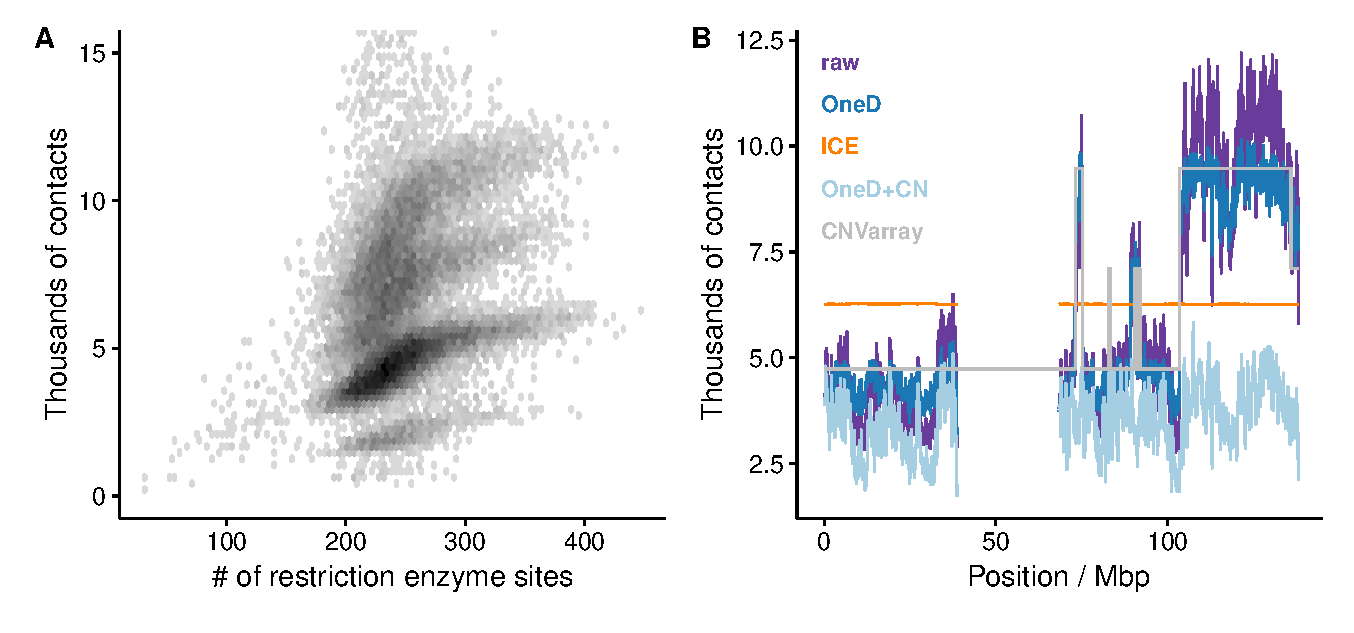
\includegraphics[width=.49\textwidth]
  {nar_figures/figure_1.eps}}
\caption{Modeling biases from the contact profile. A. Non linear
relationship between the number of restriction sites and the total number
of contacts per bin in T47D. B. Total number of contacts per bin on
chromosome 17 of T47D. The brown line represents the raw signal, the blue
line represents the signal after bias correction, the black line
represents the signal after bias and copy number (CN) correction. The long
arm of chromosome 17 (the region corresponding to 20-80 Mbp) is present in
four copies, explaining that the signal is about twice higher than for the
short arm.}
\label{fig:totals}
\end{figure}


Experimental biases affect the contact profile in a continuous but not
necessarily linear way. Figure~\ref{fig:totals}A shows the relationship
between the amount of contacts and the number of restriction enzyme sites
in T47D, a breast cancer cell line with an aberrant karyotype.  Four
clouds are visible. Each corresponds to sequences present in one to four
copies. In all of them, the relationship flattens as the number of
restriction sites increases. To capture this relationship, \textit{OneD}
fits a non-linear model between the total amount of contacts and the known
sources of bias (by default the G+C content, the number of restriction
sites and the mappability of the reads).

The experimental biases are estimated genome-wide and each cell of the
Hi-C matrix is then corrected using equation (\ref{eq:xhat}). Note that
the corrected contact profile is still proportional to the copy number.
In cancer cell lines, the contact profile corrected by \textit{OneD} is
highly correlated to the copy number estimated from an external source
(Supplementary Figure~1). Figure~\ref{fig:totals}B shows the corrected
contact profile along chromosome 17 of T47D. \textit{OneD} greatly reduces
the wiggling of the contact profile (dark blue line).

Optionally, \textit{OneD} allows the user to also correct the Hi-C signal
for the copy number. In this case, a hidden Markov model is fitted on the
corrected contact profile in order to infer the local copy number. Each
cell of the Hi-C matrix is then further corrected using equation
(\ref{eq:cnvnorm}), \textit{i.e.} it is divided by the square root of the
inferred copy number. In essence, this approach flatens the contact
profile so that it is no longer proportional to the local copy number. The
light blue line in figure~\ref{fig:totals}B shows the result of this
process. After this correction, the contact profile fluctuates around a
genome-wide constant value.

In what follows, we benchmarked \textit{OneD} and \textit{OneD} with copy
number correction (\textit{OneD+CN}) against \textit{vanilla},
\textit{ICE} \citep{imakaev2012iterative}, the \textit{KR} algorithm
\citep{knight2013fast}, \textit{caICB} \citep{wu2016computational} and the
Local Genomic Features method \citep[\textit{LGF},][]{hu2012hicnorm,
servant2012hitc}. The first four methods correct biases implicitly,
whereas the fifth method does it explicitly.

We used four metrics to compare Hi-C matrices (see Materials and Methods).
For consistency and concision, the results based on the reproducibility
score of \citet{yan2017hicspector} are shown in the main figures, and the
results based on the other metrics are shown in the Supplementary
Material.


%Given that our model is based on the total number of contacts, we reasoned
%that a preliminary test would be to check if the corrected number of
%contacts per bin reflects the copy number (as measured by an independent
%technique such as array-based copy-number segmentation). We tested the
%validity of this approach against the Catalogue Of Somatic Mutations In
%Cancer \citep[COSMIC,][]{forbes2010cosmic}. Figure \ref{fig:copy_number}
%shows the Pearson correlation between the corrected number of contacts and
%the copy number estimation for T47D and K562 (a leukemia cell line with an
%aberrant karyotype). Similar results were obtained using Spearman
%correlation (Supplementary Figure 1).  All the methods except
%\textit{OneD} decreased the agreement between the signal and the copy
%number because they partially corrected the discrepancy. In contrast,
%\textit{OneD} enhanced the conformity of the signal with the copy number.
%Not correcting for variable copy number at that stage may seem
%counter-intuitive, but the tests below will show this leads to better
%performance.
%
%
%\begin{figure}
%\centerline{\includegraphics[width=.39\textwidth]
%  {nar_figures/figure_2.eps}}
%\caption{Pearson correlation between the total number of contacts per bin
%and an independent estimation of the copy number (COSMIC). Left panel
%T47D breast cancer cell line, right panel K562 leukemia cell line.}
%\label{fig:copy_number}
%\end{figure}
%



\subsection{Aberrant karyotypes}

We first benchmarked the performance of our approach on biological
samples with an aberrant karyotype. A good normalization method should
increase the similarity between biological replicates by reducing
irrelevant experimental variance, such as batch effects, laboratory of
origin and protocol variations. Likewise, a good normalization should
increase the contrast between different samples to enhance the
biological differences.

We collected multiple Hi-C data sets obtained from T47D and K562 cells,
both with aberrant karyotypes. The first pool, referred to as the T47D data
set contained six T47D samples and two K562 samples, the second, refered
to as the K562 data set contained eight T47D samples and two T47D samples.
We compared matrices before and after normalization by different methods
(see Materials and Methods, distributions shown in Supplementary Figures~2
and 3). This gave an indication of the impact of a given normalization
method on the biological variation (differences between samples from T47D
and K562) and on the technical variation (differences among samples from
the same cell type). The results are summarized in
Figure~\ref{fig:aberrant}.

\begin{figure}
\centerline{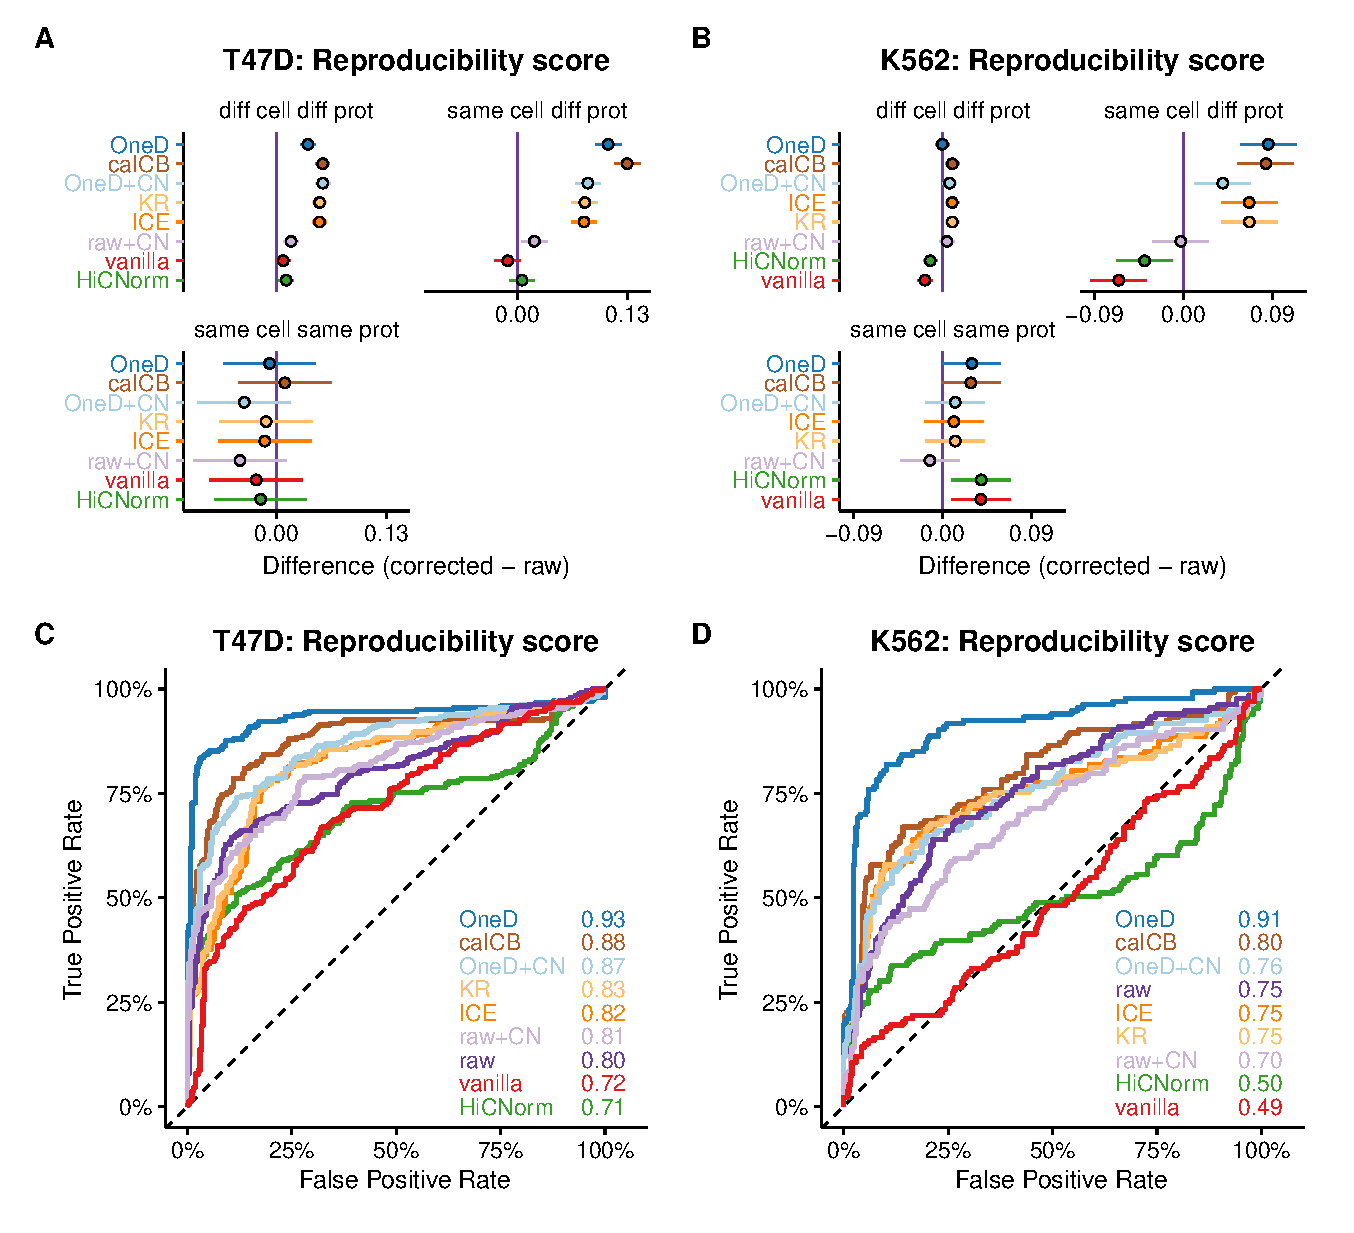
\includegraphics[width=.49\textwidth]
  {nar_figures/figure_2.eps}}
\caption{Removing biases from Hi-C on aberrant karyotypes. A and B.
Average changes compared to the raw data on the T47D and K562 data sets.
The bars represent 95\% confidence intervals centered on the mean
difference of the reproducibility score between a given correction method
and the raw data. C and D. ROC curves on the T47D and K562 sets. The areas
under the curve are indicated in the bottom right corner. The color code
is the same as in panels A and B.}
\label{fig:aberrant}
\end{figure}

On the T47D data set, the methods that increased the reproducibility
between identical cell types also increased it between different cell
types (Figures~\ref{fig:aberrant}A), meaning that none of them enhanced
exclusively the biological signal. However, the difference was most marked
for \textit{OneD} and \textit{caICB}. On the K562 data set
(figure~\ref{fig:aberrant}B), both methods increased the reproducibility
between identical cell types but not between different cell types
%Figures~\ref{fig:aberrant}B)
, which is the desired behavior of a
correction method. On both data sets, \textit{OneD+CN}, \textit{ICE} and
\textit{KR} gave inferior results, while \textit{raw+CN} (copy number
correction alone), \textit{LGF} and \textit{vanilla} were not competitive.
The conclusions were unchanged when using other metrics to compare Hi-C
matrices (Supplementary Figures~4, 5 and 6).

An important application of normalization methods in experimental setups
is to identify outliers. We thus investigated the capacity of the
different methods to help identify the samples from the other cell type
spiked in the data set. We interpreted the pairwise comparison scores as
classifier scores and summarized the results with a ROC curve
(Figures~\ref{fig:aberrant}C and D). \textit{OneD} had the largest area
under the curve in both tests, and the corresponding ROC curve was above
the others throughout. Using other metrics to compare Hi-C matrices
yielded similar results (Supplementary Figures~4, 5 and 6).

Taken together, these results show that \textit{OneD} enhances the
biological variation and reduces the noise on samples with an aberrant
karyotype.




\subsection{Normal karyotypes}

Does the performance of \textit{OneD} on aberrant karyotypes come at the
cost of decreased performance on normal karyotypes? To address this
question, we collected data from mouse B cells and embryonic stem (ES)
cells, both with a normal karyotype. The cell types were pooled in almost
equal proportions (see Supplementary Table~1) and we performe the same
tests as above using the same metrics (distributions shown in
Supplementary Figure~7)

In this test, the reproducibility between different cell types was barely
affected (Figure~\ref{fig:normal}A). All the methods increased the
reproducibility between identical cell types (except one, see below), but
only when the experimental conditions were different. This means that all
the methods were able to remove some technical biases. \textit{ICE} and
\textit{KR} showed the stongest increase in reproducibility, but
\textit{OneD}, \textit{OneD+CN}, and \textit{caICB} had competitive
performance. \textit{vanilla} and \textit{LGF} were less competitive, and
\textit{raw+CN} (copy number correction alone) performed poorly, because
it is equivalent to no normalization on diploid cells. Other metrics gave
similar results (Supplementary Figures~8, 9 and 10).

As above, we used the reproducibility score for classification and
compared the tools with a ROC curve (Figure~\ref{fig:normal}B). The
performance of the all tools were high and less variable than for
aneuploid cell lines. \textit{OneD} achieved the highest area under the
curve on this problem, but with a small margin over \textit{KR} and
\textit{ICE}. The performance of \textit{OneD+CN} was the same as that of
\textit{OneD} because copy numer correction has no effect on diploid cell
lines. Using other metrics to compare matrices gave similar results
(Supplementary Figures~8, 9 and 10).

We took advantage of the wide range of protocols used in the GM12878 set to
further investigate the performance of each method. The differences between
methods were minor and \textit{OneD} showed the greatest improvement in
reporducibility (Supplementary Figure~11).

Taken together, these results indicate that \textit{OneD} performs as well
as the best normalization methods, even with normal karyotypes.

\begin{figure}
\centerline{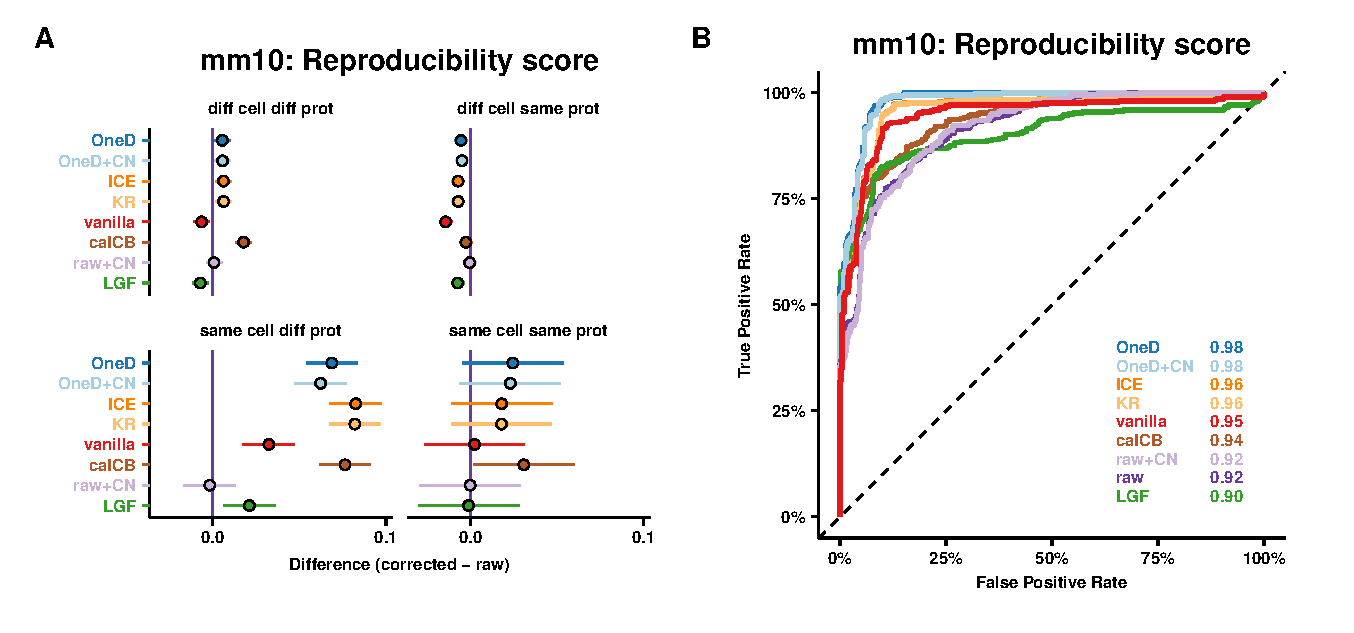
\includegraphics[width=.49\textwidth]
  {nar_figures/figure_3.eps}}
\caption{Removing biases from Hi-C on normal karyotypes. A. Average
changes compared to the raw data on the mouse data set.  B. ROC curves on
the mouse data set. The legend and color code are as in
Figure~\ref{fig:aberrant}.}
\label{fig:normal}
\end{figure}


\subsection{Copy number correction}

The results so far suggest that the copy number correction lowers the
performance of \textit{OneD}. A possible limitation in Hi-C is the absence
of ground truth. We thus used simulations to generate matrices with
defined karyotypic aberrations (see Materials and Methods) and tested the
capacity of the correction methods to distinguish different cell types
(Supplementary Figure~12). On this test, \textit{LGF} and \textit{OneD}
performed best. In comparison, \textit{OneD+CN} performed less well,
suggesting that correcting the copy number attenuates the biological
signal. This is corroborated by the fact that the copy number correction
alone has a lower performance than no correction at all. Thus, copy number
correction can indeed have side effects that lower the biological signal.

However, those conclusions are based on data sets where the karyotype is
uniform. One sometimes needs to compare samples from cells with different
karyotype, for instance in cancer samples where the karyotypes may change
through time. In such conditions, copy number correction can remove a
feature that is considered irrelevant in order to highlight other
biological differences.

To test this idea, we collected a Hi-C data set from breast cancer cell
lines and measured the reproducibility score bewteen identical cell types
after normalization with the different tools. In this case, we found that
\textit{OneD+CN} outperformed \textit{OneD} and gave the highest overall
reproducibility (Figure~\ref{fig:cnv_correction}A). Even though the
variability is high in this case, this suggests that the karyotypes of
these cells have diverged, so that the copy number correction performed by
\textit{OneD} increased the reproducibility between samples from the same
cell type.

\begin{figure}
\centerline{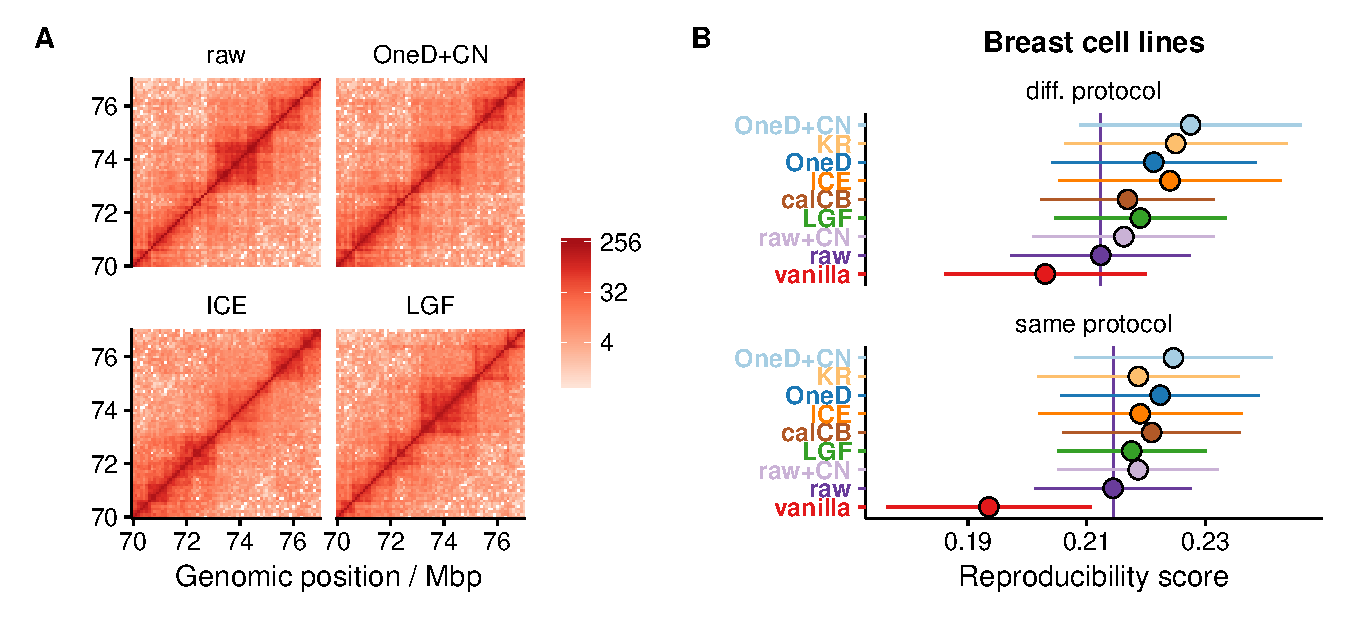
\includegraphics[width=.49\textwidth]
  {nar_figures/figure_4.eps}}
\caption{Copy number correction. A. Removing biases from Hi-C on breast
cancer cells. The reproducibility score between samples from the same
breast cancer cell type was computed after normalization. The vertical bar
shows the reproducibility score of the raw data. Shown are comparisons for
different (top) or identical (bottom) experimental conditions. B. Detail
of a Hi-C matrix normalized with different methods. The central portion
has an increased copy number, which affects normalization. \textit{ICE}
fades it away, \textit{LGF} enhances it and \textit{OneD} reduces the
signal by about half.}
\label{fig:cnv_correction}
\end{figure}

Copy number correction is also useful to give euploid-equivalent
representations of samples from aberrant karyotypes.
Figure~\ref{fig:cnv_correction}B shows an example where a region at the
center of the matrix is duplicated. \textit{ICE} overcompensated the
original bias and faded the signal almost entirely. Concomitantly, the
signal at the bottom left of the matrix was enhanced and showed a
structure that was not visible in the raw data. On the contrary,
\textit{LGF} strengthened the central region and the diagonal.
\textit{OneD} reduced the level of the central portion by a factor 2
approximately, but did not otherwise distort the main features of the
region.

In summary, \textit{OneD+CN} can improve the reproducibility of samples
with unstable karyotypes, and it can be used to obtain an
euploid-equivalent normalized matrix.


\subsection{Capture Hi-C}

Matrix-balancing methods (here \textit{ICE}, \textit{vanilla} and the
\textit{KR} algorithm) are specifically tailored for Hi-C because it is
the dominant 3C-derived technology. As a consequence, their performance is
typically lower when they are used for variants such as and Capture Hi-C
\citep{jager2015capture}. In this case, the contacts with one or more
regions of interest are enriched through direct purification, essentially
erasing all the other contacts from the Hi-C matrix. The lack of
homogeneity of the signal in such technologies makes normalization
particularly challenging.

We reasoned that \textit{OneD} should handle such cases gracefully,
because the signal is formally equivalent to an aberrant karyotype where
most of the genome is present in zero copy. We thus evaluated the
performance of \textit{OneD} on a Capture Hi-C data set at 5~kbp
resolution centered on a 6~Mbp domain of chromosome 6 in T47D cells. We
found that the reproducibility score between replicates was higher after
normalization with \textit{OneD} than with matrix-balancing methods
(figure~\ref{fig:chic}A). The performance of \textit{OneD} was only
slightly lower than the raw data, suggesting that it barely disturbs the
biological signal. Other tools were not included beause they either
crashed (\textit{caICB}) or had prohibitive run time (\textit{LGF}).

\begin{figure}
\centerline{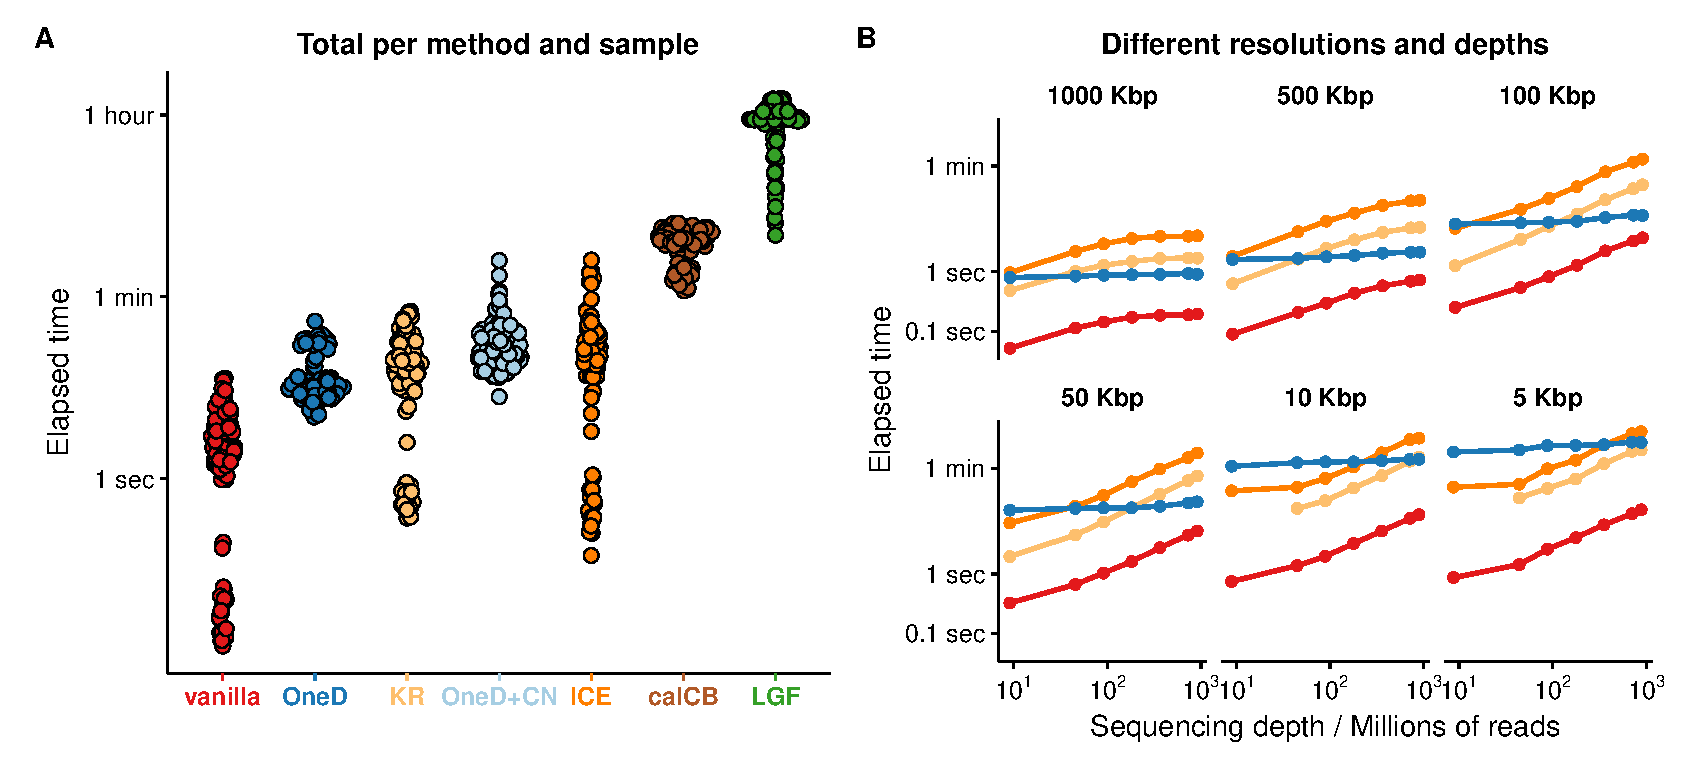
\includegraphics[width=.49\textwidth]
  {nar_figures/figure_5.eps}}
\caption{Bias removal on Capture Hi-C data A. Performance on the Capture
Hi-C data. Two replicates centered on a 6~Mbp domain on chromosome 6 in
T47D cells were normalized by the indicated tools and their
reproducibility score was computed. B. Performance on virtual Capture Hi-C
data. Two Hi-C experiments were post-processed to produce an output
similar to the Capture Hi-C experiment depicted in panel A. The signal
outside the domain on chromosome 6 was removed and the data were
normalized (capt), or the data were normalized before removing the signal
oustside the domain on chromosome 6 (full). Four matrices per method were
generated and the reproducibility score between the pairs from different
replicates were computed. Note that the scores are identical for the raw
data because in this case the matrices of the same replicate are
identical.}
\label{fig:chic}
\end{figure}

To gain additional insight, we also set up a ``virtual Capture Hi-C'' data
set by removing the signal outside the same region of chromosome 6 from
Hi-C experiments performed in the same cell type. In this setup, we could
restrict the data and then normalize, or normalize and then restrict the
data. This allowed us to probe how sensitive the methods are to the shape
of the input data. Here we found that \textit{OneD} significantly
outperformed the other methods: it featured the highest reproducibility
score between replicates with practically no influence from the shape of
the data (figure~\ref{fig:chic}B). Also, in this case, \textit{OneD}
enhanced the reproducibility bewteen replicates compared to the raw data.
This confirms the view that capture methods are a natural framework for
the statistical model underlying \textit{OneD}. In comparison,
matrix-balancing methods showed lower reproducibility between replicates,
together with more variability due to the shape of the data.

In conclusion, \textit{OneD} is suitable for removing experimental biases
from data acquired with Capture Hi-C.

\subsection{Speed}

Finally, we compared the computational speed of the different
normalization methods. \textit{vanilla} and \textit{ICE} are broadly used
because of their conceptual simplicity, ease of use and speed
\citep{imakaev2012iterative}. This is even more significant as current
explicit methods \citep{servant2012hitc} are much slower in comparison.

\textit{OneD} corrects a single variable instead of the whole matrix, and
thus estimates the model parameters much faster than previous explicit
methods. We measured the running time of the different tools on a 3.3~GHz
machine with 62 GB~RAM, always using the default parameters.
Figure~\ref{fig:times}A shows the running times of the different methods
on all the samples shown in Supplementary Figure~1 at 100~kbp resolution.
The fastest method was \textit{vanilla} and the slowest \textit{LGF}, with
an over 100-fold span between the two.

On average, \textit{OneD} was the second fastest method and it always ran in less than
1~min in the conditions of the benchmark. The copy number correction
increased the running time, but it remained under 1~min in general.
Throughout this benchmark, the memory footprint of \textit{OneD} was less
than 300 MB.  Interestingly, the running time of \textit{OneD} was much
more homogeneous than that of the other methods. The reason is that the
size of the regression problem to be solved by the \texttt{mgcv} package
is always the same at fixed resolution.

\begin{figure}
\centerline{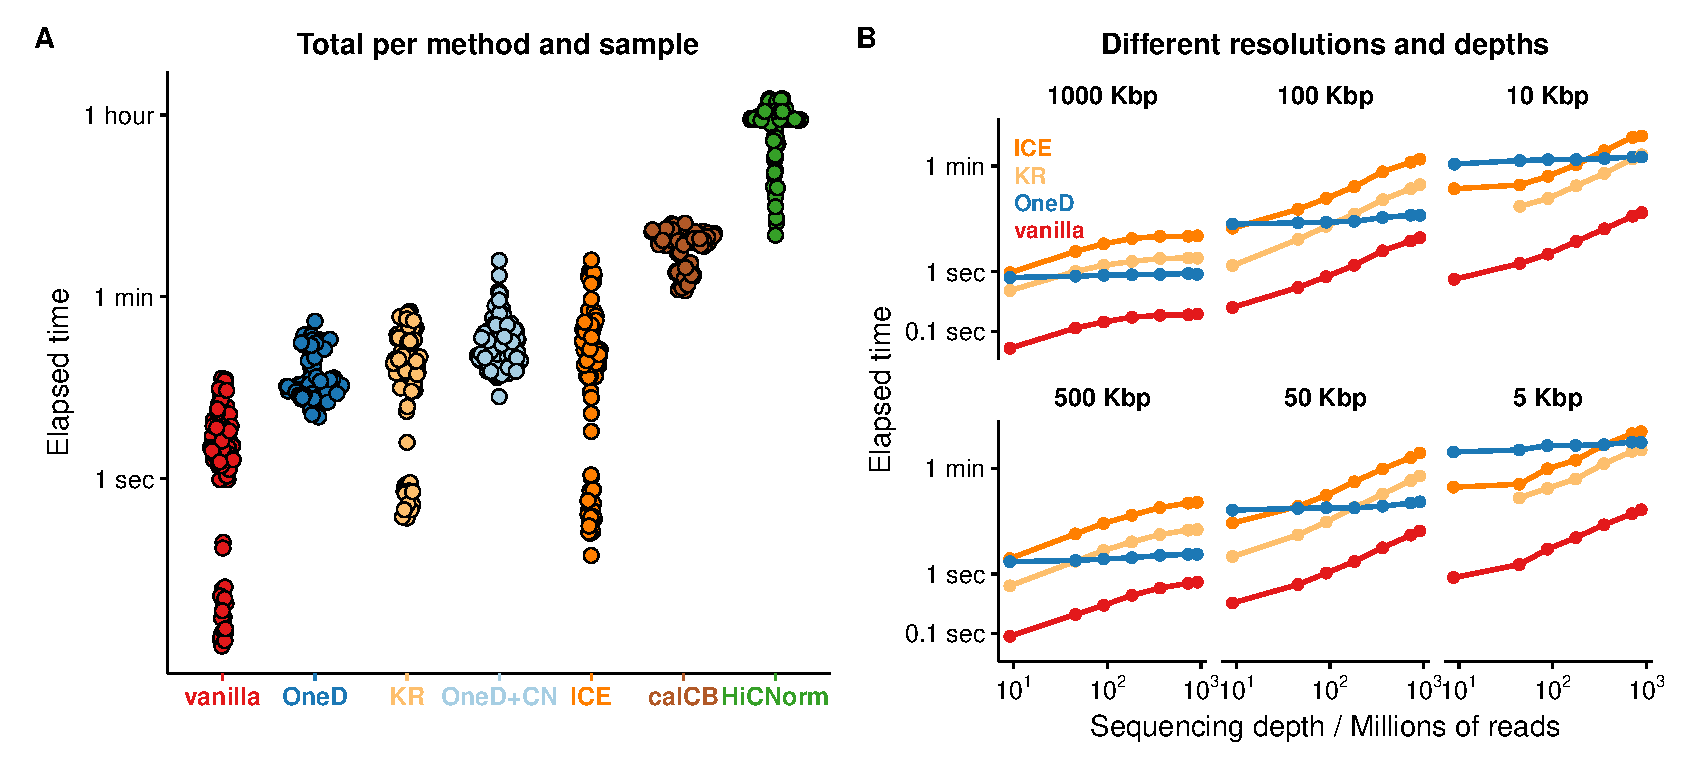
\includegraphics[width=.49\textwidth]
  {nar_figures/figure_6.eps}}
\caption{Computing time of the bias correction methods. A. Total time to
process samples listed in Supplementary Table~1 at 100~kbp resolution.
Each dot corresponds to a sample. B. Total time to process sample HIC070
at the indicated bin size and sequencing depths. Note the logarithmic
scale on the y-axis on both panels.}
\label{fig:times}
\end{figure}

To better understand these results, we also investigated the influence of
bin size and sequencing depth on the running time. We performed a
benchmark on the sample with highest sequencing depth in the data set
(HIC070, see Supplementary Table~1) at different bin sizes while
downsampling the contact matrices to mimic lower resolutions. On this
test, we included only the methods competing with \textit{OneD} in terms
of speed, \textit{i.e.} the matrix-balacing methods.
Figure~\ref{fig:times}B shows that the running time of \textit{OneD} does
not depend on the sequencing depth. Strikingly, \textit{OneD} also gives
nearly identical results at very different sequencing depths
(Supplementary Figure~13). \textit{vanilla} was the overall fastest method
and \textit{OneD} was usually faster than \textit{ICE} and \textit{KR}
at high but not at low sequencing depth. At low resolution (100~kbp) the
speed advantage of \textit{OneD} appeared from low sequencing depth, but
at high resolution reslution (5~kbp) it appeared only at high sequening
depth.

Taken together, these results show that \textit{OneD} is competitive in
terms of speed. It is particularly adapted to projects where the
sequencing depth is high, as the running time is essentially not affected.



\section{DISCUSSION}

Here we introduced \textit{OneD}, a fast computational method to normalize
Hi-C matrices. \textit{OneD} was developed ground up to address the need
to normalize data from biological samples with aberrant karyotypes, but it
applies seamlessly to the case of normal karyotypes. We showed that
\textit{OneD} performs significantly better than other methods when the
cells present karyotypic aberrations (Figure~\ref{fig:aberrant}), and that
it performs equally well as the best methods on euploid genomes
(Figure~\ref{fig:normal}). We also showed that \textit{OneD} is
approximately as fast as \textit{ICE} (Figure~\ref{fig:times}), which
makes it competitive from the point of view of computational speed.

The originality of \textit{OneD} lies in the estimation of the explicit
biases and the copy number from a single variable: the contact profile.
This allows greater running speed, while preserving a good performance on
samples with karyotypic aberrations. One of the reasons why \textit{OneD}
is able to better highlight the biological distinctions between samples is
that it only corrects the copy number if specifically requested by the
user. The impact of copy number variations on normalization is rather
opaque, especially if they are treated as implicit biases
(Figure~\ref{fig:cnv_correction}B). Treating them as explicit biases with
optional removal seems to be an overall safer strategy. In homogeneous
data sets, correcting for the copy number can blur the biological signal,
but when karyotypes are variable or unstable, it may increase the
reproducibility (Figure~\ref{fig:cnv_correction}A).

This raises the question whether variations of the copy number constitute
a biological signal or an artifact. If the biological sample contains
karytoypic aberrations, then its genome is grossly different from the
reference genome, which makes signal correction very challenging. The
proper approach would be to use the actual genome of the biological sample
as a reference to construct the contact map. However, this strategy is
presently unfeasible because assembling mammalian genomes is still a hard
problem.

Depending on the intention of the user, the effect of the copy number
should either be kept or removed. This is why \textit{OneD} does not
perform the correction by default, but allows the user to obtain a
euploid-equivalent Hi-C map computed from a hidden Markov model. The
resulting matrices have a near constant amount of contacts per bin, but
the artifacts caused by the mismatch between the genome of the sample and
the reference genome are still present (for instance, the artifacts caused
by large scale inversions are not changed in any way).


\section{CONCLUSION}

Overall, \textit{OneD} constitutes a novel computational approach to
normalize Hi-C matrices. If the karyotype of the sample is aberrant, it
enhances the biological variation.  If not, it performs at least equally
well as other methods in terms of quality and of computational speed.


\section{ACKNOWLEDGEMENTS}

We would like to thank the members of the 4DGenome Synergy project for the
fruitful discussions during project meetings. E.V. wants to acknowledge
the members of Miguel Beato's laboratory for their insights during lab
meetings.


\section{FUNDING}

This work was partially supported by the Spanish Ministry of Economy and
Competitiveness `Centro de Excelencia Severo Ochoa 2013-2017'
(SEV-2012-0208) and ACER to CRG. R.S. was supported by an EMBO Long-term
Fellowship (ALTF 1201-2014) and a Marie Curie Individual Fellowship
(H2020-MSCA-IF-2014). We received funding from the European Research
Council under the European Union's Seventh Framework Programme
(FP7/2007-2013)/ERC Synergy grant agreement 609989 (4DGenome). The content
of this manuscript reflects only the author's views and the Union is not
liable for any use that may be made of the information contained therein.

\subsubsection{Conflict of interest statement.} None declared.
\newpage

\bibliographystyle{natbib}
\bibliography{references}


\end{document}
